\section{\textit{Game Boy Advance}} \label{gba}

  O \textit{Game Boy Advance} é um vídeo game portátil lançado em 2001 pela Nintendo, possuindo tela com resolução de $240\times160$ \textit{pixels} e até 32768 cores possíveis, sistema de som estéreo PCM e processador ARM de 32 bits com memória incorporada \cite{nintendo}.

  O detalhamento de cada tipo de memória, que seguirá até o fim desta seção, tem como referência \cite{cowbite}.

  \subsection{Memória} \label{gba-memory}

    O \textit{Game Boy Advance} possui várias semelhanças com um PC como por exemplo processador, memória \textit{RAM}, ferramentas para entrada de dados e placa mãe \cite{harbour}. Ao desenvolver jogos para ambas as plataformas, porém, há uma nítida diferença em se tratando do controle do hardware por parte do programador. Ao programar em um PC, o sistema operacional fornece uma série de funções que facilitam o acesso ao hardware, enquanto no GBA, o acesso ao hardware é feito acessando diretamente uma determinada posição de memória (registrador).

    \citeonline{gbatek}, no \textit{GBATek}, classifica a memória utilizável como memória interna geral, memória interna do display e memória externa. A memória interna geral é dividida em \textit{System ROM} (BIOS), \textit{On-Board Work RAM}, \textit{On-chip Work RAM} e \textit{I/O Registers}. Já a memória interna do display divide-se em \textit{Pallete RAM}, \textit{Video RAM} (VRAM) e \textit{OBJ Attributes Memory} (OAM). Por fim, a memória externa é formada por 4 \textit{Game PAK ROM's} e uma \textit{Game PAK SRAM}. Por sua vez, o \textit{CowBite Virtual Especifications} trata essa última região de memória de forma mais geral, como \textit{Cart RAM}, e explica que ela pode ser utilizada como SRAM, \textit{Flash ROM} ou EEPROM.

    A \textit{System ROM} possui 16 \textit{KBytes} de tamanho e contém a BIOS do sistema. Essa região de memória pode ser usada somente para escrita e qualquer tentativa de leitura resultará em falha.

    A \textit{On-Board Work RAM}, citada pelo \textit{GBATek}, é tratada como \textit{External Work RAM} (EWRAM) pelo \textit{CowBite Virtual Specifications}. Ela possui 256 \textit{KBytes} de tamanho e é utilizada para inserir código e dados do jogo. Se um cabo \textit{multiboot} estiver presente quando o console for iniciado, a BIOS irá detectá-lo e automaticamente deverá transferir o código binário para essa região.

    A \textit{On-Chip Work RAM} é tratada pelo o \textit{Cowbite Virtual Specifications} como \textit{Internal Work RAM} (IWRAM) e possui 32 \textit{KBytes} de espaço. Dentre as RAM's do GBA, essa é a mais rápida. Levando em consideração que seu barramento possui 32 \textit{bits} de tamanho, enquanto o da \textit{System ROM} e da EWRAM possuem apenas 16 \textit{bits}, é recomendado que o código ARM\footnote{\textit{A32 instructions, known as Arm instructions in pre-Armv8 architectures, are 32 bits wide, and are aligned on 4-byte boundaries. A32 instructions are supported by both A-profile and R-profile architectures.} \cite{arm}} de 32 \textit{bits} seja utilizado aqui, deixando o código \textit{THUMB}\footnote{\textit{The T32 instruction set, known as Thumb in pre-Armv8 architectures, is a mixed 32- and 16-bit length instruction set that offers the designer excellent code density for minimal system memory size and cost.} \cite{arm}} para ser utilizado na \textit{System ROM} e EWRAM

    A \textit{I/O RAM}, citada anteriormente como \textit{I/O Registers}, possui 1 \textit{KByte} de extensão e é utilizada para acesso direto à memória, controle dos gráficos, do áudio e de outras funções do GBA.

    A \textit{Pallete RAM} possui 1 \textit{KByte} de tamanho e tem como função armazenar as cores de 16 \textit{bits} necessárias quando se deseja utilizar paletas de cores. Ela possui duas áreas: uma para \textit{backgrounds} e outra para \textit{sprites}. Cada uma dessas áreas pode ser utilizada como uma única paleta de cores ou como 16 paletas de 16 cores cada.

    A \textit{Video RAM} (VRAM) possui 96 \textit{KBytes} de espaço e é onde devem ser armazenados os dados gráficos do jogo para que possam ser mostrados na tela do GBA. A \textit{OBJ Attributes Memory} (OAM) possui 1 \textit{KByte} de tamanho e é utilizada para controlar as \textit{sprites} do GBA. Por fim, a \textit{Cart RAM} pode ser utilizada como \textit{SRAM}, \textit{Flash ROM} ou \textit{EEPROM}. Essa região é utilizada principalmente para salvar os dados do jogo.

  \subsection{Renderização de Vídeo}

    Segundo Vijn, o GBA possui 3 tipos de representação de gráficos:

    \begin{quote}
      \textit{All things considered, the GBA knows 3 types of graphics representations: bitmaps, tiled backgrounds and sprites. The bitmap and tiled background (also simply known as background) types affect how the whole screen is built up and as such cannot both be activated at the same time.} \cite[p. 38]{tonc}
    \end{quote}

    O GBA possui 3 modos de vídeo baseados em \textit{bitmaps} e a principal diferença entre eles está no fato de utilizarem ou não paletas de cores, no número de \textit{bits} utilizados para representar as cores e na resolução \cite{harbour}. Nesses modos, a memória de vídeo funciona como se fosse um grande \textit{bitmap}, de tal forma que cada pixel da tela é representado por uma posição na memória \cite{tonc}. A figura \ref{link-bitmap} apresenta um exemplo de \textit{bitmap}.

    \begin{figure}[H]
    \centering 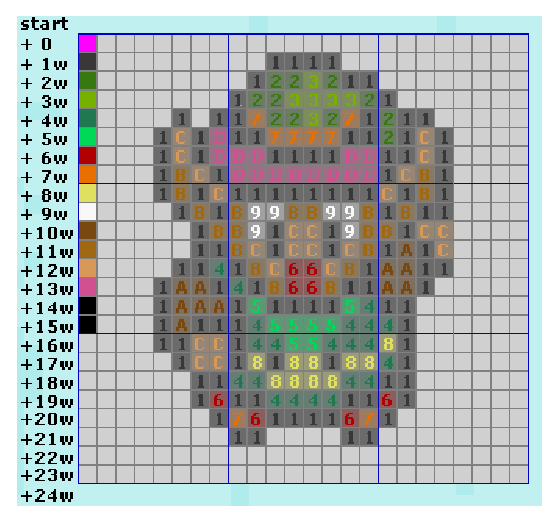
\includegraphics[keepaspectratio=true,scale=0.6]{figuras/link-bitmap.eps}
      \caption[Exemplo de \textit{bitmap} $24\times24$]
        {Exemplo de \textit{bitmap} $24\times24$. Fonte: \cite{tonc}.}
      \label{link-bitmap}
    \end{figure}

    O GBA também possui 3 modos de vídeo baseados em \textit{tiles} e a principal diferença entre eles está na quantidade de \textit{backgrounds} que podem ser utilizados em cada um dos três modos e nas operações (rotação/\textit{zoom}) que podem ser aplicadas ou não em cada um deles \cite{harbour}. Nesses modos, são construídos \textit{tiles} de $8\times8$ \textit{bits} para que posteriormente possam ser utilizados em \textit{tilemaps}, que por sua vez serão utilizados para renderizar os objetos necessários \cite{tonc}. A figura \ref{metroid-sprite} apresenta um exemplo de \textit{sprite} dividida em \textit{tiles}.

    Há ainda a camada reservada para as \textit{sprites}: ``\textit{Sprites are small ($8\times8$ to $64\times64$ pixels) graphical objects that can be transformed independently from each other and can be used in conjunction with either bitmap or background types.}'' \cite[p. 38]{tonc}

    \begin{figure}[H]
    \centering 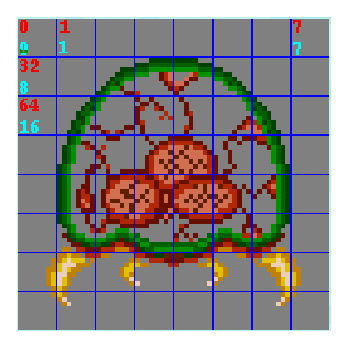
\includegraphics[keepaspectratio=true,scale=0.6]{figuras/metroid-sprite.eps}
      \caption[Exemplo de \textit{sprite} dividida em tiles]
        {Exemplo de \textit{sprite} dividida em tiles. Fonte: \cite{tonc}.}
      \label{metroid-sprite}
    \end{figure}

  \subsection{Tratamento de Input}

    O GBA possui 4 teclas direcionais e 6 botões, cujos estados podem ser acessados por meio dos 10 primeiros \textit{bits} do registrador localizado no endereço \texttt{0x4000130} \cite{gbatek}. Há ainda um outro registrador, no endereço \texttt{0x4000132}, que permite escolher quais pressionamentos de teclas geram interrupções \cite{cowbite}. A figura \ref{gba-frente} apresenta teclas e botões do GBA.

    \begin{figure}[H]
    \centering 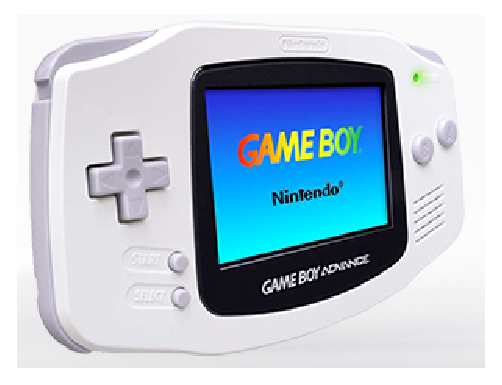
\includegraphics[keepaspectratio=true,scale=0.6]{figuras/gba-frente.eps}
      \caption[Imagem da frente do GBA mostrando teclas e botões]
        {Imagem da frente do GBA mostrando teclas e botões. Fonte: \cite{nintendo}.}
      \label{gba-frente}
    \end{figure}

  O detalhamento de cada canal de áudio, que seguirá até o fim desta seção, tem como referência \cite{gbatek}.

  \subsection{Tratamento de Áudio}

    O GBA fornece 4 canais de áudio utilizados para reproduzir tons e ruídos \cite{gbatek}. Apesar dos 4 canais de áudio, o console não possui um \textit{mixer} embutido, o que faz com que os programadores precisem escrever seus próprios \textit{mixers} ou utilizar bibliotecas de terceiros para tal propósito. Sem um \textit{mixer}, apenas um áudio pode ser tocado por vez, o que é chamado de reprodução assíncrona \cite{harbour}.

    O primeiro canal de áudio do GBA é responsável pelo tom e pelo \textit{sweep}, ele possui um registrador para controle do \textit{sweep}, um para controle da frequência, que também permite reiniciar o áudio que está sendo tocado e um registrador para controlar o volume do áudio, o padrão de onda, o \textit{envelope Step-Time} e o \textit{envelope Direction}.

    O segundo canal de áudio funciona de forma similar ao primeiro e também é responsável pelo controle do tom. Ele não possui, porém, um registrador para controle do \textit{sweep} ou do \textit{tone envelope}.

    O terceiro canal de áudio é responsável pela saída de onda e pode ser utilizado para reproduzir áudio digital. Ele também pode ser utilizado para reproduzir tons normais a depender da configuração dos registradores. O canal em questão possui um registrador para controle da RAM de onda, um para controle do comprimento e volume do áudio e um para controle da frequência, permitindo também reiniciar o áudio que está sendo tocado.

    Por fim, o quarto canal é responsável pelo ruído. Ele pode ser utilizado para reproduzir ruído branco\footnote{\textit{A musician thinks of white noise as a sound with equal intensity at all frequencies within a broad band. Some examples are the sound of thunder, the roar of a jet engine, and the noise at the stock exchange.} \cite{kuo}}, o que pode ser feito alternando randomicamente a amplitude entre alta e baixa em uma dada frequência. Também é possível modificar a função do gerador randômico de tal forma que a saída de áudio se torne mais regular, o que fornece uma capacidade limitada de reproduzir tons ao invés de ruído. Esse canal possui um registrador para controlar o volume do áudio, o \textit{Envelope Step-Time} e o \textit{Envelope Direction} e um registrador para controle da frequência, permitindo também reiniciar o áudio.
